\card{Model Checking als Verifikationstechnologie}{
	\usetikzlibrary{positioning,arrows,shapes}

\begin{tikzpicture}[every node/.style={draw},r/.style={ellipse},node distance=0.5cm,a/.style={->,>=triangle 60}]

\node(req)[r]  at (0,0) {requirements};
\node(for)[below=of req]{formalizing};
\node(prs)[r] [below=of for,text width=2.25cm]{property specification};

\node(sys) [r,right=of req,xshift=0.8cm]{system};
\node(mod) [below=of sys]{modeling};
\node(sm) [r,below=of mod]{system model};

\node(mc) [below right=of prs,xshift=-0.7cm]{model checking};
\node(sat) [r,below left=of mc]{satisfied};
\node(vio) [r,below right=of mc,text width=2.5cm]{violated +\\ counterexample};

\node(sim) [right=of sm]{simulation};
\node(loc) [r,above=of sim]{location error};

\foreach \x/\y in {req/for,for/prs,sys/mod,mod/sm,sim/loc,sm/sim}{
	\draw[a](\x)--(\y);
}
\foreach \x/\y in {prs/mc,sm/mc}{
	\draw[a](\x)|-(\y);
}

\node(p1) [right=of sat,draw=none]{};
\node(p2) [left=of vio,draw=none]{};
\node(p3) [above=of vio,draw=none]{};

\draw[a](mc.south)-|(p1.center)--(sat);
\draw[a](mc.south)-|(p2.center)--(vio);
\draw[a](vio)--(p3.center)-|(sim.south);
\end{tikzpicture}
}

\card{State-Based-Modeling: State}{
	\begin{enumerate}
		\item Charakteristik der hervorstechenden Eigenschaften eines Systems an einem bestimmten Beobachtungspunkt
		\item Konvention: ein gegebener Zustand kann solange beobachtet werden, wie die Merkmale, die von Interesse sind, unverändert bleiben
		\item Merkmale von Interesse in diskreten simultanen Softwaresystemen:
		\begin{compactenum}
			\item Kontrollpunkt ("`Programmzähler"') aller Prozesse
			\item aktuelle Werte einer lokalen und globalen Variablen am Beobachtungspunkt
			\item Inhalt aller Kommunikationskanäle im System (Nachrichten, die gesendet, aber noch nicht empfangen wurden)
		\end{compactenum}
	\item Zustände werden oft als Zustandsvektor repräsentiert (byteweise Repräsentation eines oben genannten Merkmals)
	\end{enumerate}
}

\card{State-Based-Modeling: Zustandsübergänge in diskreten Systemen}{
	\begin{enumerate}
		\item unmittelbare Veränderungen des beobachteten Merkmals des Systems
		\item repräsentiert einen Berechnungsschritt
		\item Sequenzen von Zustandsübergängen charakterisieren Berechnungen des Systems
	\end{enumerate}
	Beispiel:\\
	%\usetikzlibrary{positioning,arrows,shapes}

\begin{tikzpicture}[every node/.style={draw,ellipse}]

\node (idle) [anchor=east] at (0,0) {idle};
\node (conv) [right=of idle,anchor=west,xshift=1.3cm] {conversation};
\draw[->,>=triangle 60](idle)-- node[above,draw=none,yshift=-0.15cm] {off-hook}(conv);

\end{tikzpicture}
}

\card{State-Based-Modeling: Interne Prozesssysnchronisation}{
	\begin{enumerate}
		\item beide Telefone arbeiten völlig unabhängig von einander
		\item um das Phenomenon darzustellen, dass die beiden sich gegenseitig anrufen wollen, müssen wir eine \textbf{interne Prozesssynchronisation} hinzufügen
		\item synchrone Nachrichtenweitergabe mit den folgenden Nachrichten:
			\begin{description}
				\item[!digits] Partner anrufen
				\item[?digits] Anruf erhalten
				\item[!onhook] beenden eines Anrufes durch auflegen
				\item[?onhook] Benachrichtigung über die Beendigung des Anrufes vom Partner
			\end{description}
	\end{enumerate}
}

\card{Model Checking: System Deadlock}{
	\begin{enumerate}
		\item höchst unerwünschtes Verhalten von gleichzeitig ausgeführtem Code
		\item zeitgleich ausgeführte Prozesse warten aufeinander in einer\\kreisförmigen Wartezeit ohne "`pre-emption"' (Vorbelegung)
		\item Lösung: Prozessen erlauben die "`Entstehung"' versuchen abzubrechen, indem der Hörer aufgelegt wird
	\end{enumerate}
}

\card{Model Checking: Deadlockerfassung mit SPIN}{
algorithmischer Ansatz für das Fehlen eines Deadlocks\\im Model Checking:
	\begin{enumerate}
		\item betrachten des globalen Zustandsraum des Systems, erhalten durch das Multiplizieren der Zustandsräume der beiden Prozesse (Kartesisches Produkt der beiden Zustandsräume)
		\item systematische Suche nach dem globalen Zustandsraum für Zustände, die keinen Nachfolger haben
	\end{enumerate}
}

\card{Model Checking: Zustandsraumexploration (Erkundung) - Schritte}{
	\begin{compactenum}[\leftmargin=0pt 1.]
		\item Konstruktion eines \textit{Global State Space (GSS)} (Regeln)
		\item algorithmische Exploration des GSS (Suchen nach globalen Systemzuständen, die die Eigenschaft verletzen)
		\item Durchsuchen des GSS:
			\begin{compactenum}
				\item systematische Suche, um eine Eigenschaftsverletzung der globalen Systemzustände zu finden
				\item Strategien: DFS (benutzt Hash, Stack (benutzt um ein Counterexample zu erstellen))/BFS
				\item Eigenschaften: \textit{complete} (alle erreichbaren Zustände wurden besucht), \textit{sound} (falls ein verletzender Zustand gefunden ist, ist garantiert, dass es ein möglicher (erreichbarer) Fehler des Systems ist), \textit{if state space is finite} (Garantie, dass ein Fehler, falls vorhanden, in endlicher Zeit gefunden wird; falls kein Fehler gefunden wurde, nachdem die Sucher terminiert: Korrektheitsbeweis)
			\end{compactenum}
		\item Deadlocks sind die Zustände, die im GSS nicht mehr verlassen werden können (gerichteter Graph)
	\end{compactenum}
}

\card{Model Checking: DFS vs. BFS}{
	\begin{enumerate}
		\item Vorteile \textbf{BFS}: findet einen verletzenden Zustand immer auf dem kürzesten Weg
		\item Vorteile \textbf{DFS}: Stack enthält automatisch das \textit{Counterexample} (BFS muss den Vorgänger als zusätzliche Information speichern), Speichereffizient - muss nur einen Teil der Zustände speichern (BFS muss alle Zustände speichern)
		\item Schlussfolgerungen: \textbf{DFS} ist in unserem Fall besser, \textbf{BFS} kann nur für mäßig große Modelle verwendet werden, realistische nur mit \textbf{DFS}
	\end{enumerate}
}

\card{GSS Construction: Beispiel}{
	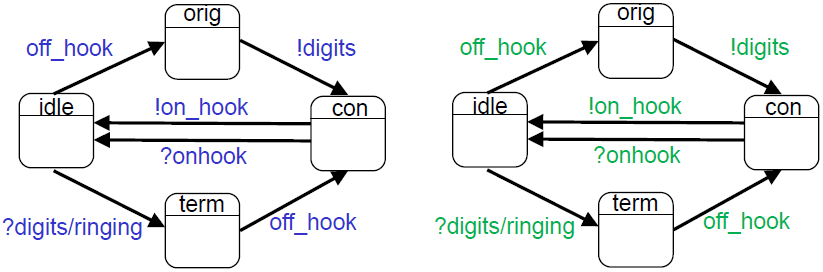
\includegraphics[width=0.8\textwidth]{pictures/phones1.png}\\
	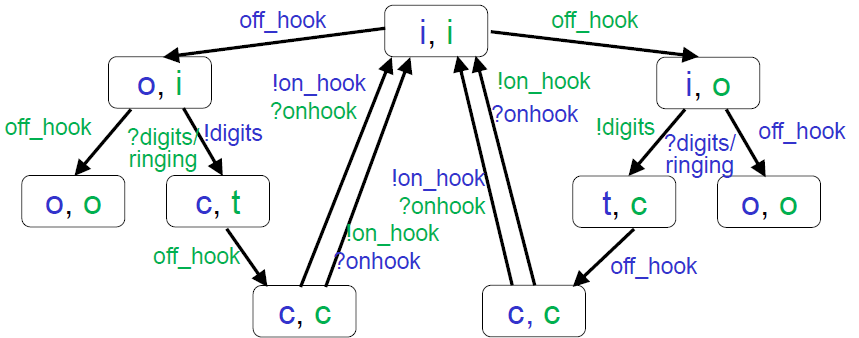
\includegraphics[width=0.8\textwidth]{pictures/phones2.png}\\
}

\card{Model Checking: Konstruktion (Berechnung) eines globalen Zustandsraums (Regeln)}{
	\begin{enumerate}
		\item Übergänge in lokalen (individuellen) Zustandsmaschinen (Statechart)
		\item Zustände im globalen Zustandsraum sind Paare der Form ($s_1,s_2$), wobei $s_1$ ein Zustand aus State Machine 1 und $s_2$ ein Zustand aus State Machine 2 ist
	\end{enumerate}
}

\card{Model Checking: Counterexample}{
	\begin{enumerate}
		\item falls eine Eigenschaftsverletzung gefunden wurde, zeigt SPIN einen Ausführungspfad vom Ausgangszustand bis zum verletzenden Zustand (hilfreich beim Debugging)
	\end{enumerate}
}

\card{Model Checking: SPIN}{
	\begin{enumerate}
		\item Syntax Check
		\item Slicing: führt eine Datenflussanalyse in Bezug auf die Eigenschaft durch, bestimmt irrelevante Teile des Modells
		\item Simulation: zufällig, interaktive oder pfadgeführte Simulation, wichtigste Debugginghilfe
		\item Verification: Model Checker, führt eine Überprüfung der Sicherheit und Lebendigkeit durch
		\item LTL Property Manager: hilft temporale Logikformeln zu bearbeiten und zu pflegen
		\item FSM View
	\end{enumerate}
}

\card{Model Checking: Never Claim}{
	\begin{enumerate}
		\item nur eine Instanz pro Promelamodell
		\item synchron mit dem Rest des Modells ausgeführt
		\item kann einen Schritt ausführen, wenn Bedinungslabel des Überganges erfüllt is im aktuellen Zustand des Promelamodells
		\item nichtdeterministischer Automat
		\item Endzustand des \textit{Never Claim} zeigt immer eine Eigenschaftsverletzung an
		\item stotternde Semantik: Endzustand wird für immer wiederholt
	\end{enumerate}
}

\card{Model Checking: Zustandsraumexplosion (Problem)}{
	\begin{enumerate}
		\item annehmen von n lokalen gleichzeitigen Prozessen (Proctypes)
		\item annehmen von K als Obergrenze für die Anzahl an Zuständen in jedem Prozess
		\item Worst Case: $K^n$
		\item Konsequenzen: Speicheranforderungen steigen exponentiell in n,\\
		Suchanstrengungen wachsen exponentiell in n\\
		Suche selbst ist Worst-Case linear
	\end{enumerate}
}

\card{Model Checking: Zustandsraumexplosion (Techniken)}{
	\begin{compactenum}
		\item On-The-Fly Search: Effizienzproblem: jeder Knoten wird zweimal besucht (Generierung der Zustände, Suche), benötigt Speicher des ganzen Zustandsraums, Gefahr: löschen von Knoten die wieder besucht werden würden; Bsp: SPIN
		\item Partial Order Reduction: reduzieren der Anzahl des erforschten\\
		Zustände und Übergänge durch Nutzung von Redundanz im Zustandsraum, Anforderungen zur Reduzierung: Eigenschaft gilt im reduzierten Zustandsraum gdw. gilt im ganzen Zustandsraum
		\item Bit-State Hashing: kein Wiederbesuchen von Zuständen $\Rightarrow$ exponentiell $\rightarrow$ linear, SPIN benutzt Hashfunktionen basierend auf Checksummenpolynomen (Jenkin's Hash), speichern eines Bits (0,1), Probleme bei Duplikaten
	\end{compactenum}
}

\card{Korrektheitsbeweis: Regeln}{
	Beweisstrategien für verschiedene Kontrollflusskonstrukte:
	\begin{enumerate}
		\item sequentielle Zusammensetzung:\\
		generelle Form: S1;S2\\
		Beweisregel:\\
		$\dfrac{\{F_1\}S_1\{F_2\},\{F_2\}S_2\{F_3\}}{\{F_1\}S_1;S_2\{F_3\}}$
		\item bedingte Aussagen (if \dots then \dots else)\\
		Beweisregel: $\dfrac{\{P \cap C\}S_1\{Q\},\{P \cap \neg C\}S_2\{Q\}}{\{P\} \text{ if C then }S_1\text{ else }S_2;\{Q\}}$
	\end{enumerate}
}